% Options for packages loaded elsewhere
\PassOptionsToPackage{unicode}{hyperref}
\PassOptionsToPackage{hyphens}{url}
%
\documentclass[
]{article}
\usepackage{lmodern}
\usepackage{amssymb,amsmath}
\usepackage{ifxetex,ifluatex}
\ifnum 0\ifxetex 1\fi\ifluatex 1\fi=0 % if pdftex
  \usepackage[T1]{fontenc}
  \usepackage[utf8]{inputenc}
  \usepackage{textcomp} % provide euro and other symbols
\else % if luatex or xetex
  \usepackage{unicode-math}
  \defaultfontfeatures{Scale=MatchLowercase}
  \defaultfontfeatures[\rmfamily]{Ligatures=TeX,Scale=1}
\fi
% Use upquote if available, for straight quotes in verbatim environments
\IfFileExists{upquote.sty}{\usepackage{upquote}}{}
\IfFileExists{microtype.sty}{% use microtype if available
  \usepackage[]{microtype}
  \UseMicrotypeSet[protrusion]{basicmath} % disable protrusion for tt fonts
}{}
\makeatletter
\@ifundefined{KOMAClassName}{% if non-KOMA class
  \IfFileExists{parskip.sty}{%
    \usepackage{parskip}
  }{% else
    \setlength{\parindent}{0pt}
    \setlength{\parskip}{6pt plus 2pt minus 1pt}}
}{% if KOMA class
  \KOMAoptions{parskip=half}}
\makeatother
\usepackage{xcolor}
\IfFileExists{xurl.sty}{\usepackage{xurl}}{} % add URL line breaks if available
\IfFileExists{bookmark.sty}{\usepackage{bookmark}}{\usepackage{hyperref}}
\hypersetup{
  pdftitle={Econometrics II - Problem 9},
  pdfauthor={William Radaic Peron},
  hidelinks,
  pdfcreator={LaTeX via pandoc}}
\urlstyle{same} % disable monospaced font for URLs
\usepackage[margin=1in]{geometry}
\usepackage{color}
\usepackage{fancyvrb}
\newcommand{\VerbBar}{|}
\newcommand{\VERB}{\Verb[commandchars=\\\{\}]}
\DefineVerbatimEnvironment{Highlighting}{Verbatim}{commandchars=\\\{\}}
% Add ',fontsize=\small' for more characters per line
\usepackage{framed}
\definecolor{shadecolor}{RGB}{248,248,248}
\newenvironment{Shaded}{\begin{snugshade}}{\end{snugshade}}
\newcommand{\AlertTok}[1]{\textcolor[rgb]{0.94,0.16,0.16}{#1}}
\newcommand{\AnnotationTok}[1]{\textcolor[rgb]{0.56,0.35,0.01}{\textbf{\textit{#1}}}}
\newcommand{\AttributeTok}[1]{\textcolor[rgb]{0.77,0.63,0.00}{#1}}
\newcommand{\BaseNTok}[1]{\textcolor[rgb]{0.00,0.00,0.81}{#1}}
\newcommand{\BuiltInTok}[1]{#1}
\newcommand{\CharTok}[1]{\textcolor[rgb]{0.31,0.60,0.02}{#1}}
\newcommand{\CommentTok}[1]{\textcolor[rgb]{0.56,0.35,0.01}{\textit{#1}}}
\newcommand{\CommentVarTok}[1]{\textcolor[rgb]{0.56,0.35,0.01}{\textbf{\textit{#1}}}}
\newcommand{\ConstantTok}[1]{\textcolor[rgb]{0.00,0.00,0.00}{#1}}
\newcommand{\ControlFlowTok}[1]{\textcolor[rgb]{0.13,0.29,0.53}{\textbf{#1}}}
\newcommand{\DataTypeTok}[1]{\textcolor[rgb]{0.13,0.29,0.53}{#1}}
\newcommand{\DecValTok}[1]{\textcolor[rgb]{0.00,0.00,0.81}{#1}}
\newcommand{\DocumentationTok}[1]{\textcolor[rgb]{0.56,0.35,0.01}{\textbf{\textit{#1}}}}
\newcommand{\ErrorTok}[1]{\textcolor[rgb]{0.64,0.00,0.00}{\textbf{#1}}}
\newcommand{\ExtensionTok}[1]{#1}
\newcommand{\FloatTok}[1]{\textcolor[rgb]{0.00,0.00,0.81}{#1}}
\newcommand{\FunctionTok}[1]{\textcolor[rgb]{0.00,0.00,0.00}{#1}}
\newcommand{\ImportTok}[1]{#1}
\newcommand{\InformationTok}[1]{\textcolor[rgb]{0.56,0.35,0.01}{\textbf{\textit{#1}}}}
\newcommand{\KeywordTok}[1]{\textcolor[rgb]{0.13,0.29,0.53}{\textbf{#1}}}
\newcommand{\NormalTok}[1]{#1}
\newcommand{\OperatorTok}[1]{\textcolor[rgb]{0.81,0.36,0.00}{\textbf{#1}}}
\newcommand{\OtherTok}[1]{\textcolor[rgb]{0.56,0.35,0.01}{#1}}
\newcommand{\PreprocessorTok}[1]{\textcolor[rgb]{0.56,0.35,0.01}{\textit{#1}}}
\newcommand{\RegionMarkerTok}[1]{#1}
\newcommand{\SpecialCharTok}[1]{\textcolor[rgb]{0.00,0.00,0.00}{#1}}
\newcommand{\SpecialStringTok}[1]{\textcolor[rgb]{0.31,0.60,0.02}{#1}}
\newcommand{\StringTok}[1]{\textcolor[rgb]{0.31,0.60,0.02}{#1}}
\newcommand{\VariableTok}[1]{\textcolor[rgb]{0.00,0.00,0.00}{#1}}
\newcommand{\VerbatimStringTok}[1]{\textcolor[rgb]{0.31,0.60,0.02}{#1}}
\newcommand{\WarningTok}[1]{\textcolor[rgb]{0.56,0.35,0.01}{\textbf{\textit{#1}}}}
\usepackage{graphicx,grffile}
\makeatletter
\def\maxwidth{\ifdim\Gin@nat@width>\linewidth\linewidth\else\Gin@nat@width\fi}
\def\maxheight{\ifdim\Gin@nat@height>\textheight\textheight\else\Gin@nat@height\fi}
\makeatother
% Scale images if necessary, so that they will not overflow the page
% margins by default, and it is still possible to overwrite the defaults
% using explicit options in \includegraphics[width, height, ...]{}
\setkeys{Gin}{width=\maxwidth,height=\maxheight,keepaspectratio}
% Set default figure placement to htbp
\makeatletter
\def\fps@figure{htbp}
\makeatother
\setlength{\emergencystretch}{3em} % prevent overfull lines
\providecommand{\tightlist}{%
  \setlength{\itemsep}{0pt}\setlength{\parskip}{0pt}}
\setcounter{secnumdepth}{-\maxdimen} % remove section numbering

\title{Econometrics II - Problem 9}
\author{William Radaic Peron}
\date{\today}

\begin{document}
\maketitle

\textbf{Ref:} IPEA Discussion Paper 230, Lecture 8 - Notes, Enders
5.1-5.3.

In this problem, we'll apply ARDL modelling to the Phillips Curve.
Namely, we'll focus on two hypothesis for the curve:

\begin{itemize}
\item \textbf{Inertial inflation.} There's a backward-looking component to any Phillips curve.
\item \textbf{Rational expectations.} The curve is forward-looking.
\end{itemize}

From these hypothesis, it is also possible to test a hybrid approach
that incorporates both a backward and a forward component.

\section{ARDL models}

Consider the following model:
\[ Y_t = \alpha + \sum_{j=0}^q \theta_j X_{t-j} + \varepsilon_t \] This
is the \emph{distributed lag} model for \(q\) lags of \(X\). Note that
\(Y_t\) has serial correlation because of its relation with \(X_{t-j}\).

An \emph{Autoregressive distributed lag} model is a combination of an
\(AR(p)\) with a \(DL(q)\):
\[ Y_t = \alpha + \sum_{i=1}^p \phi_i Y_{t-i} + \sum_{j=0}^q \theta_j X_{t-j} + \varepsilon_t \]
Or, with lag operator notation:
\[ \Phi (L) Y_t = \alpha + \Theta (L) X_t + \varepsilon_t \]

We can further define
\(\Psi := \Phi^{-1} (L) \Theta (L) = \psi_0 + \psi_1 L + ....\) This
implies that we can rewrite the ARDL(p,q) model as:
\[ Y_t = \Phi^{-1}(1)\alpha + \Psi (L) X_t + \Phi^{-1} (L) \varepsilon_t \]
Also note that we can expand this definition by letting \(X_{t,s}\) be a
matrix of \(s\) processes.

\section{Phillips Curve and its developments}

Phillips famously postulated a negative relation -- i.e., a trade-off --
between inflation rate and unemployment. We can define this curve as
follows: \[ \pi_t = \alpha - \gamma u_t, \] where \(\pi_t\) is
inflation, \(u_t\) is unemployment and \(\gamma > 0\). Note that this is
a \emph{static model}. Furthermore, note that this formulation proposes
a \emph{long term trade-off} between these variables.

Friedman and Phelps disputed the claims of these long run effects by
including \emph{expectations} in the model. The monetarist Phillips
curve asserted that inflation expectations would be formed as a function
of \emph{past inflation rates} -- i.e., under the assumption of
adaptative expectations. This model has the following representation:
\[ \pi_t = \mathbb{E}_{t-1}(\pi_t) - \gamma (u_t - \bar{u}), \] where
\(\bar{u}\) represents the natural rate of unemployment (NAIRU). This is
called the Accelerationist Phillips Curve (APC), given its
\emph{backward-looking} -- hence, inertial -- nature. Now, the model is
\emph{dynamic}, and can be translated to the ARDL framework with
\(Y_t := \pi_t, X_t := \mathbb{E}_{t-1}(\pi_t)\).

The rational expectations revolution of Lucas and Sargent, which implied
fundamental critiques to the Keynesian system, prompted a revaluation of
its framework, including the Phillips Curve. The New Keynesian Phillips
Curve (NKPC) incorporates \emph{rational expectations} in the model:
\[\pi_t = \beta \mathbb{E}_t (\pi_{t+1}) + \gamma x_t, \] where \(x_t\)
is a measure of output gap. Note that this model is essentially
\emph{forward-looking}.\\

\begin{quote}
This model implies that there is no need for gradualist policies to reduce inflation. According to the NKPC, low inflation can be achieved immediately by the central bank announcing (and the public believing) that it is committing itself to eliminating positive output gaps in the future. (IPEA, p. 11)
\end{quote}

We can interpret this model in the ARDL framework as a DL model with
\(X_t := \mathbb{E}_{t}(\pi_{t+1})\).

Some authors have also proposed a NKPC with a backward-looking element.
This is called the Hybrid Philips Curve:
\[ \pi_t = \gamma_b \pi_{t-1} + \gamma_f \mathbb{E}_t (\pi_{t+1}) + \kappa x_t. \]
This can be interpreted as an ARDL(1,1) model, with
\(X_t := \mathbb{E}_{t-1}(\pi_t)\).

\section{Estimation}

These hypothesis will now be tested with Brazilian time series data for
inflation, unemployment and inflation expectation.

\begin{Shaded}
\begin{Highlighting}[]
\CommentTok{# APC}

\NormalTok{nairu <-}\StringTok{ }\KeywordTok{hpfilter}\NormalTok{(df}\OperatorTok{$}\NormalTok{unemployment, }\DecValTok{1600}\NormalTok{, }\DataTypeTok{type =} \StringTok{'lambda'}\NormalTok{)}

\KeywordTok{plot}\NormalTok{(nairu)}
\end{Highlighting}
\end{Shaded}

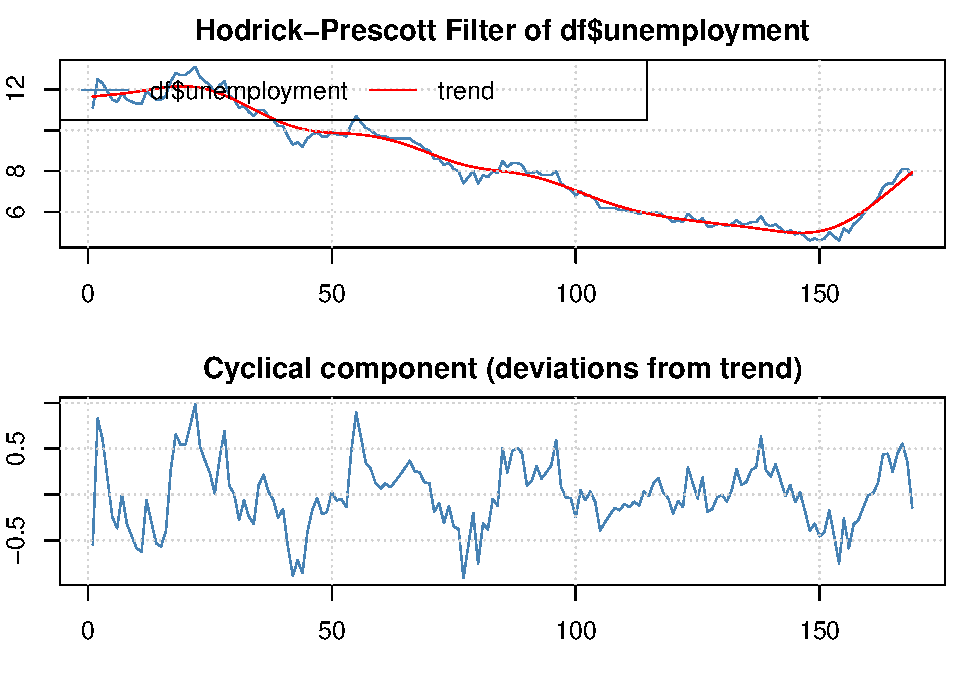
\includegraphics{Econo2_P9_files/figure-latex/ardl estimation-1.pdf}

\begin{Shaded}
\begin{Highlighting}[]
\NormalTok{nairu_trend <-}\StringTok{ }\NormalTok{nairu}\OperatorTok{$}\NormalTok{trend}

\NormalTok{u_dev <-}\StringTok{ }\NormalTok{df}\OperatorTok{$}\NormalTok{unemployment }\OperatorTok{-}\StringTok{ }\NormalTok{nairu_trend}

\NormalTok{df}\OperatorTok{$}\NormalTok{u_dev =}\StringTok{ }\NormalTok{u_dev}

\NormalTok{exp_lag =}\StringTok{ }\NormalTok{dplyr}\OperatorTok{::}\KeywordTok{lag}\NormalTok{(df}\OperatorTok{$}\NormalTok{exp_IPCA, }\DataTypeTok{k=}\DecValTok{1}\NormalTok{)}

\NormalTok{df}\OperatorTok{$}\NormalTok{exp_lag =}\StringTok{ }\NormalTok{exp_lag}

\NormalTok{df2 =}\StringTok{ }\NormalTok{df[}\DecValTok{2}\OperatorTok{:}\KeywordTok{length}\NormalTok{(df}\OperatorTok{$}\NormalTok{IPCA),]}

\NormalTok{auto_apc <-}\StringTok{ }\KeywordTok{auto_ardl}\NormalTok{(IPCA }\OperatorTok{~}\StringTok{ }\NormalTok{exp_lag }\OperatorTok{+}\StringTok{ }\NormalTok{u_dev, }\DataTypeTok{data =}\NormalTok{ df2, }\DataTypeTok{max_order =} \DecValTok{12}\NormalTok{)}
\end{Highlighting}
\end{Shaded}

\begin{verbatim}
## Warning: The `x` argument of `as_tibble.matrix()` must have unique column names if `.name_repair` is omitted as of tibble 2.0.0.
## Using compatibility `.name_repair`.
## This warning is displayed once every 8 hours.
## Call `lifecycle::last_warnings()` to see where this warning was generated.
\end{verbatim}

\begin{Shaded}
\begin{Highlighting}[]
\KeywordTok{summary}\NormalTok{(auto_apc}\OperatorTok{$}\NormalTok{best_model)}
\end{Highlighting}
\end{Shaded}

\begin{verbatim}
## 
## Time series regression with "ts" data:
## Start = 13, End = 168
## 
## Call:
## dynlm::dynlm(formula = full_formula, data = data, start = start, 
##     end = end)
## 
## Residuals:
##      Min       1Q   Median       3Q      Max 
## -0.50165 -0.13225 -0.00937  0.15074  0.53030 
## 
## Coefficients:
##                Estimate Std. Error t value Pr(>|t|)    
## (Intercept)    -0.20593    0.15248  -1.351 0.179360    
## L(IPCA, 1)      1.36220    0.09409  14.477  < 2e-16 ***
## L(IPCA, 2)     -0.25922    0.15632  -1.658 0.099869 .  
## L(IPCA, 3)     -0.15454    0.14216  -1.087 0.279168    
## L(IPCA, 4)      0.03670    0.14287   0.257 0.797728    
## L(IPCA, 5)     -0.00382    0.13884  -0.028 0.978097    
## L(IPCA, 6)      0.01040    0.13806   0.075 0.940101    
## L(IPCA, 7)     -0.28244    0.13509  -2.091 0.038651 *  
## L(IPCA, 8)      0.23050    0.13592   1.696 0.092482 .  
## L(IPCA, 9)      0.16376    0.13237   1.237 0.218452    
## L(IPCA, 10)    -0.19093    0.07024  -2.718 0.007531 ** 
## exp_lag         0.19976    0.14986   1.333 0.185038    
## L(exp_lag, 1)  -0.21667    0.27641  -0.784 0.434648    
## L(exp_lag, 2)   0.11636    0.29766   0.391 0.696551    
## L(exp_lag, 3)   0.05002    0.27272   0.183 0.854787    
## L(exp_lag, 4)  -0.11920    0.26643  -0.447 0.655394    
## L(exp_lag, 5)   0.13768    0.26194   0.526 0.600115    
## L(exp_lag, 6)  -0.08363    0.25155  -0.332 0.740129    
## L(exp_lag, 7)  -0.13985    0.24522  -0.570 0.569529    
## L(exp_lag, 8)   0.19974    0.24368   0.820 0.414009    
## L(exp_lag, 9)   0.43565    0.23764   1.833 0.069222 .  
## L(exp_lag, 10) -0.88295    0.23142  -3.815 0.000216 ***
## L(exp_lag, 11)  0.21339    0.21510   0.992 0.323144    
## L(exp_lag, 12)  0.23022    0.10933   2.106 0.037301 *  
## u_dev           0.17855    0.10235   1.744 0.083618 .  
## L(u_dev, 1)    -0.17677    0.12056  -1.466 0.145184    
## L(u_dev, 2)     0.17243    0.12087   1.427 0.156279    
## L(u_dev, 3)    -0.02066    0.11855  -0.174 0.861926    
## L(u_dev, 4)    -0.15435    0.11717  -1.317 0.190220    
## L(u_dev, 5)    -0.10897    0.11954  -0.912 0.363813    
## L(u_dev, 6)     0.09109    0.11789   0.773 0.441180    
## L(u_dev, 7)     0.09352    0.11742   0.796 0.427340    
## L(u_dev, 8)    -0.07746    0.11673  -0.664 0.508205    
## L(u_dev, 9)    -0.07030    0.11578  -0.607 0.544857    
## L(u_dev, 10)    0.19848    0.10036   1.978 0.050240 .  
## ---
## Signif. codes:  0 '***' 0.001 '**' 0.01 '*' 0.05 '.' 0.1 ' ' 1
## 
## Residual standard error: 0.2358 on 121 degrees of freedom
## Multiple R-squared:  0.9945, Adjusted R-squared:  0.993 
## F-statistic: 643.1 on 34 and 121 DF,  p-value: < 2.2e-16
\end{verbatim}

\begin{Shaded}
\begin{Highlighting}[]
\KeywordTok{Box.test}\NormalTok{(auto_apc}\OperatorTok{$}\NormalTok{best_model}\OperatorTok{$}\NormalTok{residuals)}
\end{Highlighting}
\end{Shaded}

\begin{verbatim}
## 
##  Box-Pierce test
## 
## data:  auto_apc$best_model$residuals
## X-squared = 0.020209, df = 1, p-value = 0.887
\end{verbatim}

\begin{Shaded}
\begin{Highlighting}[]
\KeywordTok{AIC}\NormalTok{(auto_apc}\OperatorTok{$}\NormalTok{best_model)}
\end{Highlighting}
\end{Shaded}

\begin{verbatim}
## [1] 24.24382
\end{verbatim}

\begin{Shaded}
\begin{Highlighting}[]
\KeywordTok{BIC}\NormalTok{(auto_apc}\OperatorTok{$}\NormalTok{best_model)}
\end{Highlighting}
\end{Shaded}

\begin{verbatim}
## [1] 134.0386
\end{verbatim}

\begin{Shaded}
\begin{Highlighting}[]
\CommentTok{# APC as DL of order 1}

\NormalTok{apc1 <-}\StringTok{ }\KeywordTok{dynlm}\NormalTok{(IPCA }\OperatorTok{~}\StringTok{ }\NormalTok{exp_lag }\OperatorTok{+}\StringTok{ }\NormalTok{u_dev, }\DataTypeTok{data =}\NormalTok{ df2)}

\KeywordTok{summary}\NormalTok{(apc1)}
\end{Highlighting}
\end{Shaded}

\begin{verbatim}
## 
## Time series regression with "numeric" data:
## Start = 1, End = 168
## 
## Call:
## dynlm(formula = IPCA ~ exp_lag + u_dev, data = df2)
## 
## Residuals:
##     Min      1Q  Median      3Q     Max 
## -4.0369 -1.0285 -0.3057  0.7819  5.8672 
## 
## Coefficients:
##             Estimate Std. Error t value Pr(>|t|)    
## (Intercept) -2.83045    0.48542  -5.831 2.83e-08 ***
## exp_lag      1.73784    0.08576  20.265  < 2e-16 ***
## u_dev        1.43364    0.33701   4.254 3.51e-05 ***
## ---
## Signif. codes:  0 '***' 0.001 '**' 0.01 '*' 0.05 '.' 0.1 ' ' 1
## 
## Residual standard error: 1.53 on 165 degrees of freedom
## Multiple R-squared:  0.7139, Adjusted R-squared:  0.7105 
## F-statistic: 205.9 on 2 and 165 DF,  p-value: < 2.2e-16
\end{verbatim}

\begin{Shaded}
\begin{Highlighting}[]
\KeywordTok{Box.test}\NormalTok{(apc1}\OperatorTok{$}\NormalTok{residuals) }\CommentTok{# Modelo claramente inconsistente}
\end{Highlighting}
\end{Shaded}

\begin{verbatim}
## 
##  Box-Pierce test
## 
## data:  apc1$residuals
## X-squared = 130.33, df = 1, p-value < 2.2e-16
\end{verbatim}

\begin{Shaded}
\begin{Highlighting}[]
\CommentTok{# NKPC}

\NormalTok{auto_nkpc <-}\StringTok{ }\KeywordTok{auto_ardl}\NormalTok{(IPCA }\OperatorTok{~}\StringTok{ }\NormalTok{exp_IPCA }\OperatorTok{+}\StringTok{ }\NormalTok{u_dev, }\DataTypeTok{data =}\NormalTok{ df, }\DataTypeTok{max_order =} \DecValTok{18}\NormalTok{)}

\KeywordTok{summary}\NormalTok{(auto_nkpc}\OperatorTok{$}\NormalTok{best_model) }\CommentTok{# Unit root?}
\end{Highlighting}
\end{Shaded}

\begin{verbatim}
## 
## Time series regression with "ts" data:
## Start = 15, End = 169
## 
## Call:
## dynlm::dynlm(formula = full_formula, data = data, start = start, 
##     end = end)
## 
## Residuals:
##      Min       1Q   Median       3Q      Max 
## -0.37515 -0.10114 -0.00144  0.10024  0.42758 
## 
## Coefficients:
##                  Estimate Std. Error t value Pr(>|t|)    
## (Intercept)     -0.240062   0.126758  -1.894 0.060824 .  
## L(IPCA, 1)       1.350684   0.085512  15.795  < 2e-16 ***
## L(IPCA, 2)      -0.184944   0.138564  -1.335 0.184677    
## L(IPCA, 3)      -0.244035   0.120283  -2.029 0.044847 *  
## L(IPCA, 4)       0.042681   0.119997   0.356 0.722745    
## L(IPCA, 5)       0.024477   0.118250   0.207 0.836391    
## L(IPCA, 6)       0.082208   0.118457   0.694 0.489123    
## L(IPCA, 7)      -0.340537   0.117336  -2.902 0.004462 ** 
## L(IPCA, 8)       0.249078   0.122336   2.036 0.044107 *  
## L(IPCA, 9)       0.020930   0.122176   0.171 0.864289    
## L(IPCA, 10)     -0.060628   0.117853  -0.514 0.607961    
## L(IPCA, 11)      0.155070   0.115509   1.342 0.182150    
## L(IPCA, 12)     -0.458104   0.113047  -4.052 9.39e-05 ***
## L(IPCA, 13)      0.400469   0.111369   3.596 0.000482 ***
## L(IPCA, 14)     -0.104736   0.058148  -1.801 0.074366 .  
## exp_IPCA         0.601175   0.116501   5.160 1.08e-06 ***
## L(exp_IPCA, 1)  -0.685972   0.229083  -2.994 0.003385 ** 
## L(exp_IPCA, 2)   0.073614   0.259025   0.284 0.776784    
## L(exp_IPCA, 3)  -0.029816   0.258443  -0.115 0.908360    
## L(exp_IPCA, 4)   0.340617   0.256786   1.326 0.187385    
## L(exp_IPCA, 5)  -0.324089   0.230055  -1.409 0.161680    
## L(exp_IPCA, 6)   0.290928   0.218800   1.330 0.186334    
## L(exp_IPCA, 7)  -0.250743   0.212432  -1.180 0.240363    
## L(exp_IPCA, 8)  -0.078165   0.215093  -0.363 0.716990    
## L(exp_IPCA, 9)   0.321380   0.218641   1.470 0.144393    
## L(exp_IPCA, 10)  0.176315   0.216452   0.815 0.417047    
## L(exp_IPCA, 11) -0.711509   0.216809  -3.282 0.001376 ** 
## L(exp_IPCA, 12)  0.229051   0.199822   1.146 0.254125    
## L(exp_IPCA, 13)  0.170695   0.101511   1.682 0.095444 .  
## u_dev           -0.006651   0.093741  -0.071 0.943567    
## L(u_dev, 1)     -0.069862   0.108958  -0.641 0.522716    
## L(u_dev, 2)      0.120614   0.102093   1.181 0.239941    
## L(u_dev, 3)     -0.002564   0.101930  -0.025 0.979980    
## L(u_dev, 4)     -0.133487   0.100473  -1.329 0.186687    
## L(u_dev, 5)     -0.128222   0.101271  -1.266 0.208093    
## L(u_dev, 6)      0.180646   0.100089   1.805 0.073784 .  
## L(u_dev, 7)     -0.031687   0.099571  -0.318 0.750901    
## L(u_dev, 8)     -0.013898   0.098087  -0.142 0.887583    
## L(u_dev, 9)     -0.119316   0.098170  -1.215 0.226768    
## L(u_dev, 10)     0.089325   0.097712   0.914 0.362590    
## L(u_dev, 11)     0.126947   0.098010   1.295 0.197902    
## L(u_dev, 12)     0.196699   0.096418   2.040 0.043696 *  
## L(u_dev, 13)    -0.343949   0.084819  -4.055 9.29e-05 ***
## ---
## Signif. codes:  0 '***' 0.001 '**' 0.01 '*' 0.05 '.' 0.1 ' ' 1
## 
## Residual standard error: 0.194 on 112 degrees of freedom
## Multiple R-squared:  0.9963, Adjusted R-squared:  0.9949 
## F-statistic: 715.4 on 42 and 112 DF,  p-value: < 2.2e-16
\end{verbatim}

\begin{Shaded}
\begin{Highlighting}[]
\KeywordTok{adf.test}\NormalTok{(df2}\OperatorTok{$}\NormalTok{IPCA) }\CommentTok{# UNIT ROOT!!!!!!!!!!!!!!!!!!!!!!!!!!!!!!!}
\end{Highlighting}
\end{Shaded}

\begin{verbatim}
## 
##  Augmented Dickey-Fuller Test
## 
## data:  df2$IPCA
## Dickey-Fuller = -2.6908, Lag order = 5, p-value = 0.288
## alternative hypothesis: stationary
\end{verbatim}

\begin{Shaded}
\begin{Highlighting}[]
\CommentTok{######## Correcting for unit root ############}

\NormalTok{df3 =}\StringTok{ }\KeywordTok{data.frame}\NormalTok{(}\KeywordTok{diff}\NormalTok{(df}\OperatorTok{$}\NormalTok{IPCA), }\KeywordTok{diff}\NormalTok{(df}\OperatorTok{$}\NormalTok{exp_IPCA), df2}\OperatorTok{$}\NormalTok{u_dev)}

\KeywordTok{colnames}\NormalTok{(df3) =}\StringTok{ }\KeywordTok{c}\NormalTok{(}\StringTok{"IPCA"}\NormalTok{, }\StringTok{"exp_IPCA"}\NormalTok{, }\StringTok{"u_dev"}\NormalTok{)}

\NormalTok{diff_lag =}\StringTok{ }\NormalTok{dplyr}\OperatorTok{::}\KeywordTok{lag}\NormalTok{(df3}\OperatorTok{$}\NormalTok{exp_IPCA, }\DecValTok{1}\NormalTok{)}

\NormalTok{df3}\OperatorTok{$}\NormalTok{diff_lag =}\StringTok{ }\NormalTok{diff_lag}

\NormalTok{df4 =}\StringTok{ }\NormalTok{df3[}\DecValTok{2}\OperatorTok{:}\KeywordTok{length}\NormalTok{(df3}\OperatorTok{$}\NormalTok{IPCA),]}

\CommentTok{# APC}

\NormalTok{auto_apc_diff <-}\StringTok{  }\KeywordTok{auto_ardl}\NormalTok{(IPCA }\OperatorTok{~}\StringTok{ }\NormalTok{diff_lag }\OperatorTok{+}\StringTok{ }\NormalTok{u_dev, }\DataTypeTok{data =}\NormalTok{ df4, }\DataTypeTok{max_order =} \DecValTok{24}\NormalTok{)}

\KeywordTok{summary}\NormalTok{(auto_apc_diff}\OperatorTok{$}\NormalTok{best_model)}
\end{Highlighting}
\end{Shaded}

\begin{verbatim}
## 
## Time series regression with "ts" data:
## Start = 18, End = 167
## 
## Call:
## dynlm::dynlm(formula = full_formula, data = data, start = start, 
##     end = end)
## 
## Residuals:
##      Min       1Q   Median       3Q      Max 
## -0.41343 -0.10932  0.00661  0.09394  0.58493 
## 
## Coefficients:
##                  Estimate Std. Error t value Pr(>|t|)    
## (Intercept)      0.010941   0.018254   0.599 0.550277    
## L(IPCA, 1)       0.409004   0.105330   3.883 0.000185 ***
## L(IPCA, 2)       0.088896   0.112047   0.793 0.429432    
## L(IPCA, 3)       0.119181   0.114087   1.045 0.298704    
## L(IPCA, 4)       0.110875   0.109923   1.009 0.315575    
## L(IPCA, 5)      -0.006091   0.107789  -0.057 0.955050    
## L(IPCA, 6)       0.060649   0.090617   0.669 0.504854    
## L(IPCA, 7)      -0.258467   0.086586  -2.985 0.003564 ** 
## L(IPCA, 8)       0.127535   0.089633   1.423 0.157887    
## L(IPCA, 9)       0.058985   0.091137   0.647 0.518977    
## L(IPCA, 10)     -0.017815   0.089833  -0.198 0.843201    
## L(IPCA, 11)      0.137300   0.083879   1.637 0.104796    
## L(IPCA, 12)     -0.266226   0.089314  -2.981 0.003610 ** 
## L(IPCA, 13)      0.037546   0.090901   0.413 0.680463    
## L(IPCA, 14)     -0.099533   0.086609  -1.149 0.253207    
## L(IPCA, 15)      0.191537   0.087305   2.194 0.030560 *  
## L(IPCA, 16)      0.001053   0.086328   0.012 0.990289    
## L(IPCA, 17)     -0.009501   0.074321  -0.128 0.898535    
## diff_lag         0.249735   0.156337   1.597 0.113329    
## L(diff_lag, 1)  -0.157402   0.170257  -0.924 0.357453    
## L(diff_lag, 2)  -0.146646   0.175684  -0.835 0.405868    
## L(diff_lag, 3)   0.080162   0.171792   0.467 0.641784    
## L(diff_lag, 4)   0.053050   0.174345   0.304 0.761547    
## L(diff_lag, 5)   0.119037   0.177688   0.670 0.504453    
## L(diff_lag, 6)   0.258261   0.176193   1.466 0.145844    
## L(diff_lag, 7)  -0.261561   0.169356  -1.544 0.125640    
## L(diff_lag, 8)   0.189110   0.149533   1.265 0.208929    
## L(diff_lag, 9)   0.284296   0.144779   1.964 0.052347 .  
## L(diff_lag, 10) -0.283618   0.151988  -1.866 0.064964 .  
## L(diff_lag, 11) -0.294228   0.154530  -1.904 0.059782 .  
## L(diff_lag, 12)  0.191864   0.155691   1.232 0.220712    
## L(diff_lag, 13) -0.198643   0.149325  -1.330 0.186453    
## L(diff_lag, 14)  0.151608   0.119171   1.272 0.206256    
## u_dev            0.007234   0.114981   0.063 0.949963    
## L(u_dev, 1)     -0.221264   0.129559  -1.708 0.090773 .  
## L(u_dev, 2)      0.111406   0.127527   0.874 0.384436    
## L(u_dev, 3)      0.102516   0.126804   0.808 0.420745    
## L(u_dev, 4)     -0.021851   0.125640  -0.174 0.862280    
## L(u_dev, 5)     -0.204757   0.126623  -1.617 0.109014    
## L(u_dev, 6)      0.216744   0.117440   1.846 0.067913 .  
## L(u_dev, 7)     -0.062466   0.119477  -0.523 0.602249    
## L(u_dev, 8)      0.014275   0.118463   0.121 0.904325    
## L(u_dev, 9)     -0.112848   0.114714  -0.984 0.327621    
## L(u_dev, 10)     0.140497   0.114542   1.227 0.222853    
## L(u_dev, 11)     0.074526   0.114624   0.650 0.517065    
## L(u_dev, 12)     0.270649   0.113429   2.386 0.018912 *  
## L(u_dev, 13)    -0.296732   0.112686  -2.633 0.009800 ** 
## L(u_dev, 14)    -0.019484   0.117377  -0.166 0.868494    
## L(u_dev, 15)    -0.241873   0.117920  -2.051 0.042867 *  
## L(u_dev, 16)     0.169188   0.106435   1.590 0.115084    
## ---
## Signif. codes:  0 '***' 0.001 '**' 0.01 '*' 0.05 '.' 0.1 ' ' 1
## 
## Residual standard error: 0.2132 on 100 degrees of freedom
## Multiple R-squared:  0.8526, Adjusted R-squared:  0.7804 
## F-statistic: 11.81 on 49 and 100 DF,  p-value: < 2.2e-16
\end{verbatim}

\begin{Shaded}
\begin{Highlighting}[]
\NormalTok{n =}\StringTok{ }\DecValTok{12}
\NormalTok{x =}\StringTok{ }\KeywordTok{matrix}\NormalTok{(}\OtherTok{NA}\NormalTok{, }\DataTypeTok{nrow =}\NormalTok{ n, }\DataTypeTok{ncol =} \DecValTok{1}\NormalTok{)}

\ControlFlowTok{for}\NormalTok{ (i }\ControlFlowTok{in}\NormalTok{ (}\DecValTok{1}\OperatorTok{:}\NormalTok{n)) \{}
  
\NormalTok{  auto_apc_diff <-}\StringTok{ }\KeywordTok{auto_ardl}\NormalTok{(IPCA }\OperatorTok{~}\StringTok{ }\NormalTok{diff_lag }\OperatorTok{+}\StringTok{ }\NormalTok{u_dev, }\DataTypeTok{data =}\NormalTok{ df4, }\DataTypeTok{max_order =}\NormalTok{ i)}
  
\NormalTok{  x[i,] =}\StringTok{ }\KeywordTok{Box.test}\NormalTok{(auto_apc_diff}\OperatorTok{$}\NormalTok{best_model}\OperatorTok{$}\NormalTok{residuals)}\OperatorTok{$}\NormalTok{p.value}
  
\NormalTok{\}}


\CommentTok{# NKPC}


\NormalTok{auto_nkpc_diff <-}\StringTok{ }\KeywordTok{auto_ardl}\NormalTok{(IPCA }\OperatorTok{~}\StringTok{ }\NormalTok{u_dev }\OperatorTok{|}\StringTok{ }\NormalTok{exp_IPCA, }\DataTypeTok{data =}\NormalTok{ df3, }\DataTypeTok{max_order =} \DecValTok{18}\NormalTok{)}

\KeywordTok{summary}\NormalTok{(auto_nkpc_diff}\OperatorTok{$}\NormalTok{best_model)}
\end{Highlighting}
\end{Shaded}

\begin{verbatim}
## 
## Time series regression with "ts" data:
## Start = 19, End = 168
## 
## Call:
## dynlm::dynlm(formula = full_formula, data = data, start = start, 
##     end = end)
## 
## Residuals:
##      Min       1Q   Median       3Q      Max 
## -0.84193 -0.13569 -0.01028  0.14147  0.56659 
## 
## Coefficients:
##               Estimate Std. Error t value Pr(>|t|)    
## (Intercept)  -0.005060   0.020142  -0.251 0.802125    
## L(IPCA, 1)    0.509132   0.089594   5.683 1.08e-07 ***
## L(IPCA, 2)   -0.012886   0.104356  -0.123 0.901953    
## L(IPCA, 3)    0.116841   0.101546   1.151 0.252360    
## L(IPCA, 4)    0.105208   0.098757   1.065 0.289042    
## L(IPCA, 5)   -0.026791   0.098619  -0.272 0.786383    
## L(IPCA, 6)    0.027351   0.097234   0.281 0.779015    
## L(IPCA, 7)   -0.112602   0.088553  -1.272 0.206182    
## L(IPCA, 8)    0.063236   0.089340   0.708 0.480546    
## L(IPCA, 9)   -0.039058   0.080590  -0.485 0.628883    
## L(IPCA, 10)   0.043902   0.076831   0.571 0.568881    
## L(IPCA, 11)  -0.045146   0.076777  -0.588 0.557718    
## L(IPCA, 12)  -0.404506   0.082443  -4.906 3.20e-06 ***
## L(IPCA, 13)   0.194478   0.087748   2.216 0.028709 *  
## L(IPCA, 14)  -0.101528   0.091232  -1.113 0.268175    
## L(IPCA, 15)   0.208424   0.089401   2.331 0.021540 *  
## L(IPCA, 16)   0.079960   0.090906   0.880 0.380980    
## L(IPCA, 17)  -0.009173   0.090564  -0.101 0.919501    
## L(IPCA, 18)  -0.128494   0.075047  -1.712 0.089657 .  
## u_dev        -0.010612   0.123057  -0.086 0.931435    
## L(u_dev, 1)  -0.227780   0.142390  -1.600 0.112510    
## L(u_dev, 2)   0.169796   0.140662   1.207 0.229952    
## L(u_dev, 3)   0.152551   0.141213   1.080 0.282356    
## L(u_dev, 4)  -0.040788   0.137601  -0.296 0.767464    
## L(u_dev, 5)  -0.303975   0.134514  -2.260 0.025786 *  
## L(u_dev, 6)   0.056251   0.137073   0.410 0.682324    
## L(u_dev, 7)  -0.101813   0.126234  -0.807 0.421657    
## L(u_dev, 8)   0.179746   0.124871   1.439 0.152835    
## L(u_dev, 9)  -0.062434   0.123264  -0.507 0.613503    
## L(u_dev, 10)  0.107862   0.124115   0.869 0.386695    
## L(u_dev, 11)  0.048279   0.122524   0.394 0.694310    
## L(u_dev, 12)  0.199816   0.122730   1.628 0.106339    
## L(u_dev, 13) -0.263087   0.120391  -2.185 0.030970 *  
## L(u_dev, 14)  0.103658   0.121815   0.851 0.396634    
## L(u_dev, 15) -0.333328   0.126655  -2.632 0.009703 ** 
## L(u_dev, 16) -0.013391   0.134179  -0.100 0.920681    
## L(u_dev, 17)  0.096555   0.132828   0.727 0.468808    
## L(u_dev, 18)  0.098262   0.116650   0.842 0.401393    
## exp_IPCA      0.521329   0.136527   3.818 0.000222 ***
## ---
## Signif. codes:  0 '***' 0.001 '**' 0.01 '*' 0.05 '.' 0.1 ' ' 1
## 
## Residual standard error: 0.2401 on 111 degrees of freedom
## Multiple R-squared:  0.7925, Adjusted R-squared:  0.7215 
## F-statistic: 11.16 on 38 and 111 DF,  p-value: < 2.2e-16
\end{verbatim}

\begin{Shaded}
\begin{Highlighting}[]
\KeywordTok{Box.test}\NormalTok{(auto_nkpc_diff}\OperatorTok{$}\NormalTok{best_model}\OperatorTok{$}\NormalTok{residuals)}
\end{Highlighting}
\end{Shaded}

\begin{verbatim}
## 
##  Box-Pierce test
## 
## data:  auto_nkpc_diff$best_model$residuals
## X-squared = 0.40611, df = 1, p-value = 0.524
\end{verbatim}

\begin{Shaded}
\begin{Highlighting}[]
\NormalTok{nkpc_dyn <-}\StringTok{ }\KeywordTok{dynlm}\NormalTok{(IPCA }\OperatorTok{~}\StringTok{ }\NormalTok{exp_IPCA }\OperatorTok{+}\StringTok{ }\NormalTok{u_dev, }\DataTypeTok{data =}\NormalTok{ df3)}

\KeywordTok{summary}\NormalTok{(nkpc_dyn)}
\end{Highlighting}
\end{Shaded}

\begin{verbatim}
## 
## Time series regression with "numeric" data:
## Start = 1, End = 168
## 
## Call:
## dynlm(formula = IPCA ~ exp_IPCA + u_dev, data = df3)
## 
## Residuals:
##      Min       1Q   Median       3Q      Max 
## -2.61527 -0.17231  0.01181  0.24129  2.06516 
## 
## Coefficients:
##             Estimate Std. Error t value Pr(>|t|)    
## (Intercept)  0.01222    0.03659   0.334 0.738822    
## exp_IPCA     0.51091    0.08887   5.749 4.24e-08 ***
## u_dev       -0.35898    0.10400  -3.452 0.000707 ***
## ---
## Signif. codes:  0 '***' 0.001 '**' 0.01 '*' 0.05 '.' 0.1 ' ' 1
## 
## Residual standard error: 0.4739 on 165 degrees of freedom
## Multiple R-squared:  0.2366, Adjusted R-squared:  0.2273 
## F-statistic: 25.57 on 2 and 165 DF,  p-value: 2.124e-10
\end{verbatim}

\begin{Shaded}
\begin{Highlighting}[]
\KeywordTok{Box.test}\NormalTok{(nkpc_dyn}\OperatorTok{$}\NormalTok{residuals)}
\end{Highlighting}
\end{Shaded}

\begin{verbatim}
## 
##  Box-Pierce test
## 
## data:  nkpc_dyn$residuals
## X-squared = 71.621, df = 1, p-value < 2.2e-16
\end{verbatim}

\begin{Shaded}
\begin{Highlighting}[]
\CommentTok{# HPC }

\NormalTok{hpc_dyn <-}\StringTok{ }\KeywordTok{dynlm}\NormalTok{(IPCA }\OperatorTok{~}\StringTok{ }\NormalTok{exp_IPCA }\OperatorTok{+}\StringTok{ }\KeywordTok{L}\NormalTok{(IPCA, }\DecValTok{1}\NormalTok{) }\OperatorTok{+}\StringTok{ }\NormalTok{u_dev, }\DataTypeTok{data =}\NormalTok{ df3)}

\KeywordTok{summary}\NormalTok{(hpc_dyn)}
\end{Highlighting}
\end{Shaded}

\begin{verbatim}
## Warning in summary.lm(hpc_dyn): essentially perfect fit: summary may be
## unreliable
\end{verbatim}

\begin{verbatim}
## 
## Time series regression with "numeric" data:
## Start = 1, End = 168
## 
## Call:
## dynlm(formula = IPCA ~ exp_IPCA + L(IPCA, 1) + u_dev, data = df3)
## 
## Residuals:
##        Min         1Q     Median         3Q        Max 
## -1.136e-15 -3.240e-18  4.370e-18  1.270e-17  1.012e-16 
## 
## Coefficients:
##               Estimate Std. Error    t value Pr(>|t|)    
## (Intercept)  4.051e-18  7.073e-18  5.730e-01    0.568    
## exp_IPCA     1.651e-16  1.882e-17  8.773e+00 2.15e-15 ***
## L(IPCA, 1)   1.000e+00  1.504e-17  6.647e+16  < 2e-16 ***
## u_dev       -1.121e-17  2.081e-17 -5.390e-01    0.591    
## ---
## Signif. codes:  0 '***' 0.001 '**' 0.01 '*' 0.05 '.' 0.1 ' ' 1
## 
## Residual standard error: 9.158e-17 on 164 degrees of freedom
## Multiple R-squared:      1,  Adjusted R-squared:      1 
## F-statistic: 1.929e+33 on 3 and 164 DF,  p-value: < 2.2e-16
\end{verbatim}

\begin{Shaded}
\begin{Highlighting}[]
\KeywordTok{Box.test}\NormalTok{(hpc_dyn}\OperatorTok{$}\NormalTok{residuals)}
\end{Highlighting}
\end{Shaded}

\begin{verbatim}
## 
##  Box-Pierce test
## 
## data:  hpc_dyn$residuals
## X-squared = 0.34931, df = 1, p-value = 0.5545
\end{verbatim}

\begin{Shaded}
\begin{Highlighting}[]
\CommentTok{# The results suggest that inflation is both forward and backward looking.}
\end{Highlighting}
\end{Shaded}

\end{document}
